%compiling with XeLaTeX
\documentclass[digital, %colors on
			   %print,  %for printing
			   %twoside, %turn off for digital version
			   openright, %chapter always start on the right page
			   parskip=half,
			   11pt]{mythesis}

\usepackage{bbold}


\begin{document}
\pagestyle{plain}

\section*{The Quark Propagator DSE}
The Dyson-Schwinger equation for the quark propagator, a.k.a. the quark gap equation, relates the inverse full quark propagator $\Gamma^{(2)}_{q\bar{q}}(p)$ to its classical counterpart $S^{(2)}_{q\bar{q}}(p)$, the respective quark and gluon propagators and the classical and full quark-gluon vertices $\Gamma^{(3)}_{q\bar{q}A}(p)$. It can be formulated in terms of diagrams as follows:
 \begin{align}
\bigg(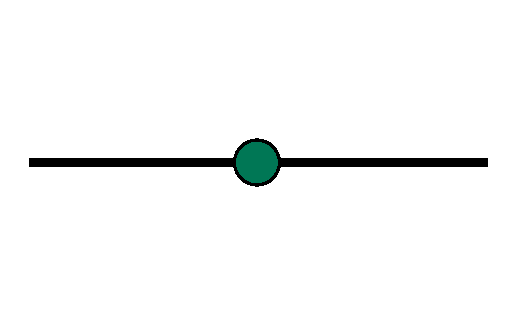
\includegraphics[scale=0.4, valign=c]{diagram/full_quark_propagator}\bigg)^{-1} = 
\bigg(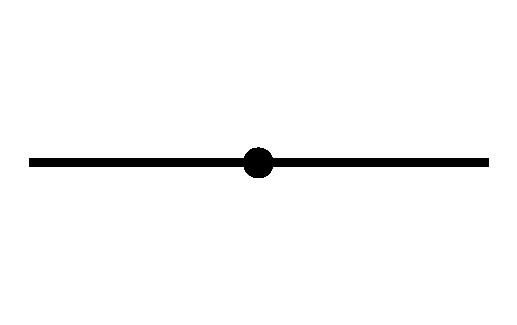
\includegraphics[scale=0.4, valign=c]{diagram/bare_quark_propagator.pdf}\bigg)^{-1} - 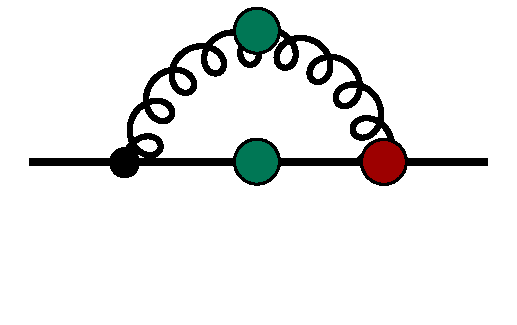
\includegraphics[scale=0.4, valign=c]{diagram/quark_self_energy}
\end{align}
 Here, green (red) blobs denote full propagators (vertices), black blobs denote classical vertices. Schematically this translates to:
 \begin{equation}
 	\Gamma^{(2)}_{q\bar{q}}(p) = S^{(2)}_{q\bar{q}}(p) + Z_1^f g_s \int_q G_{AA}(q)(-i\gamma)G_{q\bar{q}}(p+q)\Gamma^{(3)}_{q\bar{q}A}(p+q, -p).
 \end{equation}
 We suppressed all Lorenz and color indices for convenience. Since in our work, we will use a classical vertex approximation, $\Gamma^{(3)}_{q\bar{q}A}(p) \equiv S^{(3)}_{q\bar{q}A}(p)$, we won't go into details about the wave function renormalization of the quark-gluon-vertex $Z_1^f$. The two relevant renormalization constants, the wave function renormalization $Z_2$ and the mass renormalization $Z_{m_q}$ of the quark enter the gap equation via $S^{(2)}_{q\bar{q}}(p)$, i.\,e. 
 \begin{equation}
 	S^{(2)}_{q\bar{q}}(p) = iZ_2\slashed{p} + Z_{m_q}m_q,
 \end{equation}
 where $m_q$ denotes the bare current quark mass. \\
 \color{MScRed} Random question: Where does the $i$ come from??\normalcolor\\
 The full gluon and quark propagators in the Landau gauge, $\xi = 0$, are given by
 \begin{align}
 G_{AA,\mu\nu}^{ab}(p)	&= \delta^{ab} \Pi_{\bot}^{\mu\nu}G_{A}(p)\\
  G_{q\bar{q}}^{ab}(p)	&= \delta^{ab} G_{q}(p)
 \end{align}
with
\begin{align}
 G_{A}(p)	&= Z_A^{-1}(p)\frac{1}{p^2}\\
  G_{q}(p)	&= Z_q^{-1}(p)\frac{1}{i\slashed{p} + M_q(p)}.
  \end{align} \\
 \color{MScRed} In our calculation we need to replace these definitions  with the spectral representations of the respective propagators. \normalcolor\\

With all these definitions in mind we can formulate the \enquote{standard} form of the gap equation as follows:
\begin{equation}
Z_{q}(p)\left[i \slashed{p}+M_{q}(p)\right]=Z_{2} i \slashed{p}+Z_{m_{q}} m_{q}+\Sigma(p)
\end{equation}
 The next step is to project the gap equation onto its Dirac vector and scalar parts by multiplying it with either $\mathbb{1}$ or $\slashed{p}$ and performing the corresponding traces. This leaves us with a set of coupled DSEs for $Z_q(p)$ and $M_q(p)$:
 \begin{align}
 Z_q(p)p^2 &= Z_2p^2 - Z_1^f \operatorname{Tr}\left[i\slashed{p}\Sigma(p)\right]\\
  M_q(p) &= Z_q^{-1}(p)\left( Z_{m_q}m_q + Z_1^f \operatorname{Tr}\left[\Sigma(p)\right]\right)
 \end{align}

 
 
 
\end{document}